\chapter{The Proteome Profiling module}
\label{chap:protprof}

The Proteome Profiling modules is designed to identify differentially expressed protein under various experimental conditions. A typical example is to compare the effect of two substance over protein expression using whole cell lysates.

\section{Definitions}

Before explaining in detail the interface of the module and how does the module works, lets make clear the meaning of some terms that will be used in the following paragraphs.

\phantomsection
\begin{itemize}
	\item \textit{Detected protein}: any protein detected in any of the mass spectrometry experiments including the control experiments.
	\item \textit{Relevant proteins}: a detected protein with a Score value above a user defined threshold (see page \pageref{par:protprofScoreValue}).
\end{itemize}

\section{The input files}

The Proteome Profiling module requires only one input file. This Data file must follow the guidelines specified in \autoref{sec:dataFile}. In short, the Data file must have a tabular format with tab separated columns and the name of the columns are expected as first row. All columns given as input in section Column numbers of Region \num{2} of the interface must be present in the Data file.

\section{The interface}

The window of the Proteome Profiling module is divided in four regions (\autoref{fig:protprofMainWindow}). 

Region \num{1} contains four buttons allowing users to quickly delete all provided input and start a new analysis. The Clear all button will delete all user provided input and will empty the list box in Region \num{3}. The Clear files button will delete all values in section Files of Region \num{2} and will empty the list box in Region \num{3}. The Clear values button will delete all values in section Values of Region \num{2}. Finally, the Clear columns button will delete all values in section Column numbers of Region \num{2}. 

Region \num{2} contains the fields where users provide the information needed in order to perform the post-processing of the Data file. The section Files of Region \num{2} will provide the path to the Data and Output files. It contains three buttons. 

\num{1}.- The Data file button allows users to browse the file system and select a Data file. Only .txt files can be selected here. Once the Data file is selected, the name of the columns in the file will be shown in the list box of Region \num{3}. If the path to the Data file is typed in, the display of the name of the columns in Region \num{3} can be triggered by pressing the Enter key in the keyboard while the Data file entry box has the focus of the keyboard.

\num{2}.- The Output folder\label{par:protprofOutFolder} button allows users to browse the file system and select the location of the folder that will contain the output. By default, UMSAP will create a ProtProf folder inside the selected Output folder to save all the generated results. If only the name of the output folder is given, the output folder will be created in the same folder containing the Data file. If this field is left empty, then the ProtProf folder will be created in the same folder containing the Data file. If the selected Output folder already contains a ProtProf folder, then the current date and time to the seconds will be added to the name in order to avoid overwriting the files from previous analyses.

\num{3}.- The Output name button does nothing but the text box to its right allows users to specify the name of the files that will be generated during the analysis. If this field is left empty, then the name protprof will be used for the output files. 

\begin{figure}[h]
	\centering
	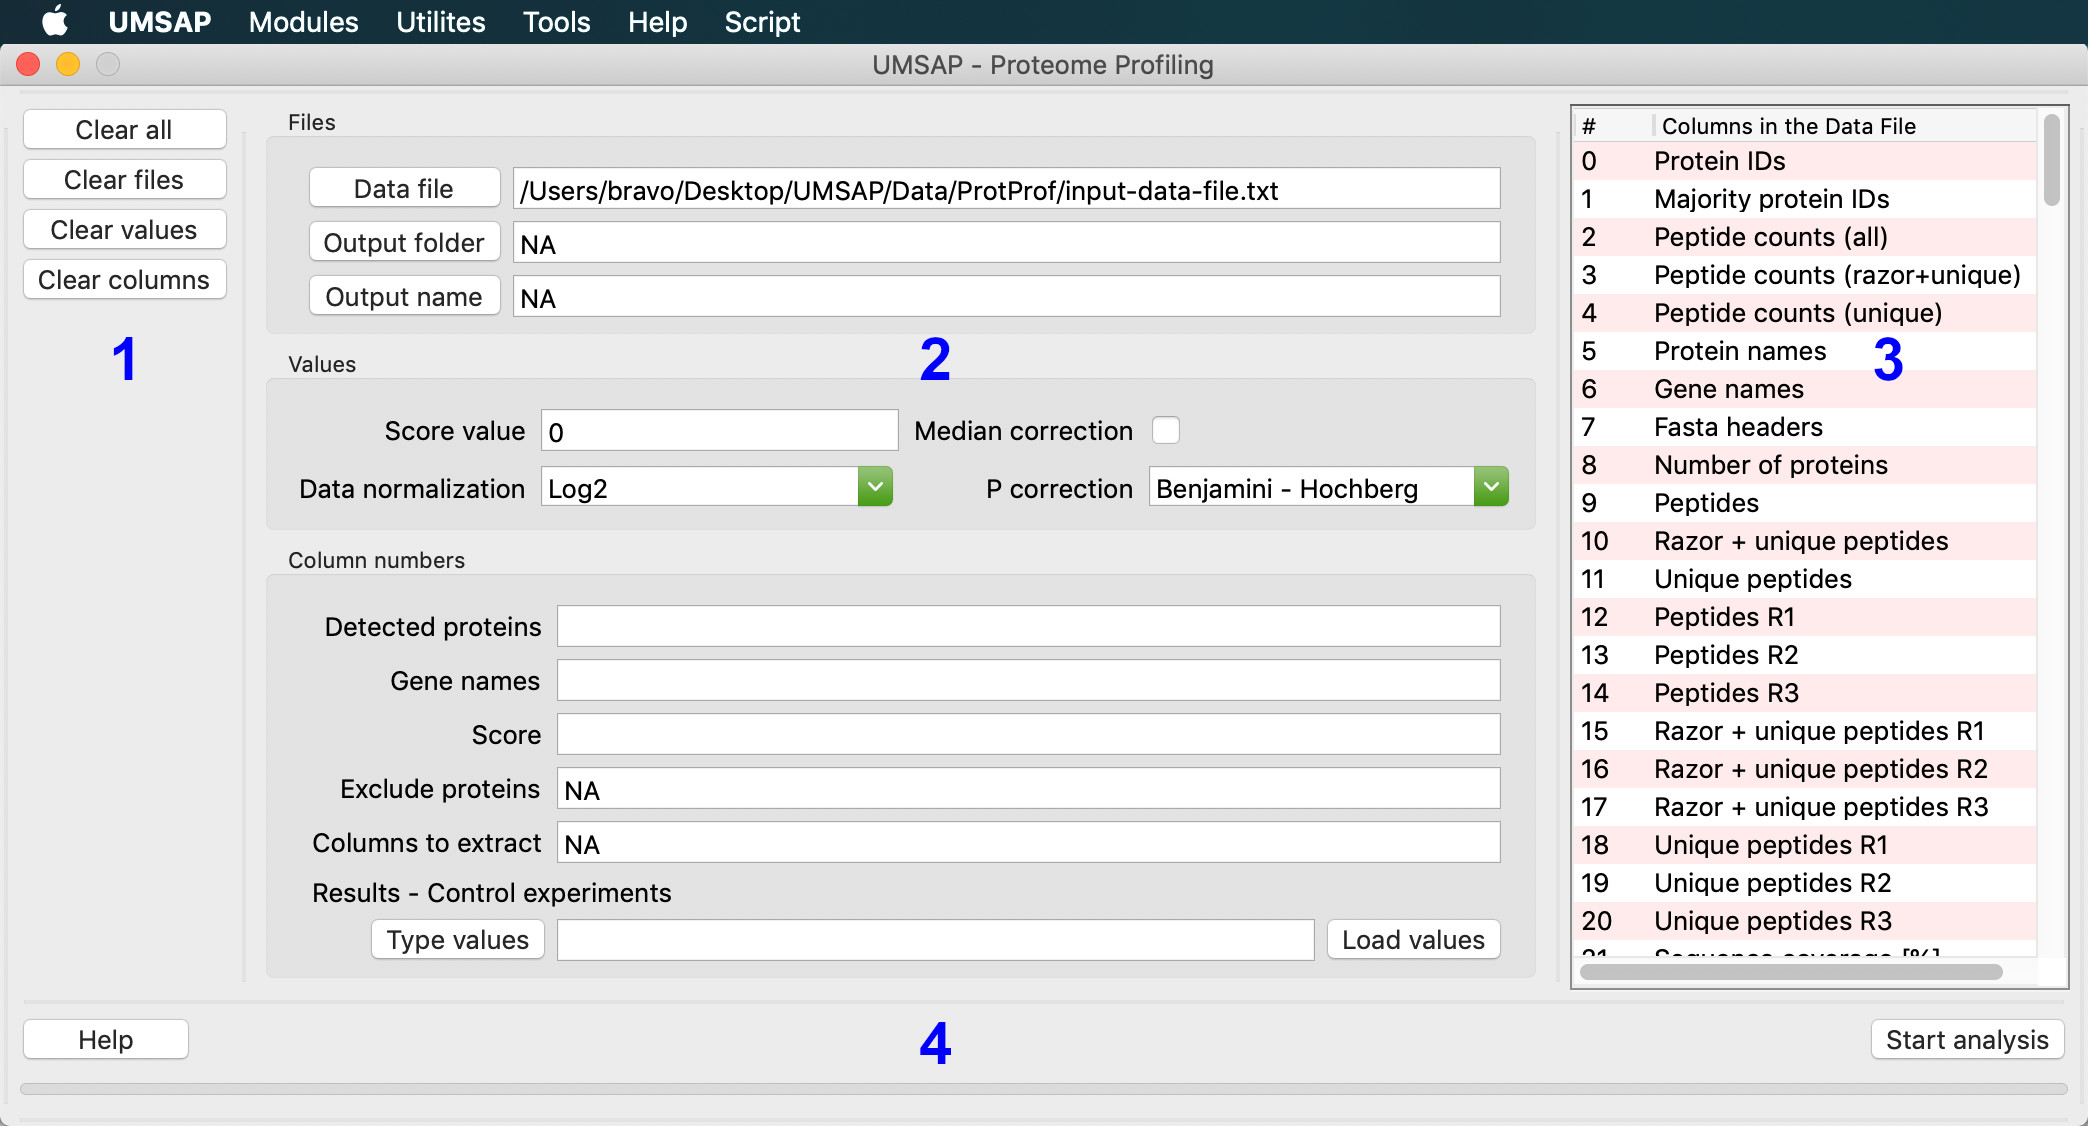
\includegraphics[width=0.7\textwidth]{./IMAGES/MOD-PROTPROF/protprof-mod.jpg}
	\caption[The Proteome Profiling module window]{\textbf{The Proteome Profiling module window.} This window allows users to performed a proteome profiling analysis. Optional parameters default to NA when the window is created. The rest of the parameters must be provided by the user.} 
	\label{fig:protprofMainWindow}
	\vspace{-5pt} 	
\end{figure} 

The section Values of Region \num{2} of the interface contains four parameters. Here, users provide information about how the Data file should be processed.

\phantomsection
\num{1}.- The parameter Score value\label{par:protprofScoreValue} allows users to define a threshold value above which the detected proteins will be considered as relevant. The Score value is an indicator of how reliable was the detection of the protein during the MS experiments. The value given to UMSAP depends on the program generating the Data file. Only one real number equal or greater than zero will be accepted as a valid input here. A value of zero means all detected proteins will be treated as relevant proteins.

\num{2}.-  The parameter Data normalization allows selecting the normalization procedure to be performed before running the analysis of the data in the Data file. Currently, only a $\log_2$ normalization is possible but this will be expanded to include quantile, variance stabilization and local regression normalization, among other methods. 

\num{3}.- The parameter Median correction indicates whether to apply a median correction to protein intensities in each experiment. The main advantage of this correction is to get symmetric volcano plots.

\num{4}.- The parameters P correction allows selecting the correction method for the p values calculated during the analysis. 

The section Column numbers of Region \num{2} contains six parameters. Here, users provide the column numbers in the Data file from where UMSAP will get the information needed to perform the analysis of the module. All columns specified in this section must be present in the Data file. Users must be aware that Python starts counting from \num{0}. Therefore, the number of the columns in the Data file starts from \num{0} and not from \num{1}. The column numbers displayed in the list box of Region \num{3} after the Data file is selected can be directly used for the values of the parameters. 

\num{1}.- The parameter Detected proteins allows users to specify the column in the Data file containing the protein identifiers found in the Data file. Only one integer number equal or greater than zero will be accepted here. 

\num{2}.- The parameter Gene names allows users to specify the column in the Data file containing the gene names of the proteins found during the MS experiments. Only one integer number equal or greater than zero will be accepted here. 

\num{3}.- The parameter Score allows to specify the column in the Data file containing the Score values.  It is in this column where the program will look for the values to be compared against the Score threshold given in section Values of Region \num{2} of the interface. Only one integer number equal or greater than zero will be accepted here. 

\num{4}.- The parameter Exclude proteins allows to specify several columns in the Data file. Proteins found in these columns will be excluded form the analysis. The module assumes that these columns contains numeric values and values greater than zero indicate that the respective protein must be eliminated from the analysis. Only integer numbers equal or greater than zero will be accepted here. A value of NA means that all proteins will be considered during the analysis. 

\num{5}.- The parameter Columns to extract\label{par:protprofColumnExtract} allows users to specify which columns in the Data file will be copy to the shorter version of the Data file, see page \pageref{subsec:utilShortDF} for more details. A range of columns may be specified as \numrange[range-phrase = --]{4}{10} with both numbers included in the range. Any number of columns may be specified here. Only integer numbers equal or greater than zero will be accepted. A value of NA means no shorter version of the Data files will be created.

\num{6}.-  \label{par:protprofResultControl}The parameter Results - Control experiments allows users to specify the columns in the Data file containing the results of the experiments. There are two ways to provide the information for this parameter. Users can load the values from a .txt file using the Load values button or use the Type values button to call a helper window, see \autoref{fig:protprofResControlWindow}. Duplicate column numbers are not allowed here.

The helper window is divided in four Regions. Region \num{1} allows to define the number of conditions and relevant points analyzed, to define the kind of control experiment performed and to create the matrix in Region \num{2}. The fields Names allow to input the names for the conditions and relevant points. A comma separated list of names is expected here. In the case of the name of the control experiment only one name is expected. If left empty default name values will be used. Each text field in Region \num{2} should contain the column numbers containing the MS results for the given experiment. The values for the text fields should be positive integer numbers or a range of integers, e.g. \numrange[range-phrase=--]{60}{62} or NA for empty experiments. Fields left empty are set to NA when the values are exported to the window of the module. The column numbers can be seen in the list box in Region \num{3}. Selected entries in the list box can be copied and then pasted to the text fields using the right mouse button or the Tools menu. Region \num{4} contains two buttons to Cancel or to Export the values to the window of the module.  

\begin{figure}[h]
	\centering
	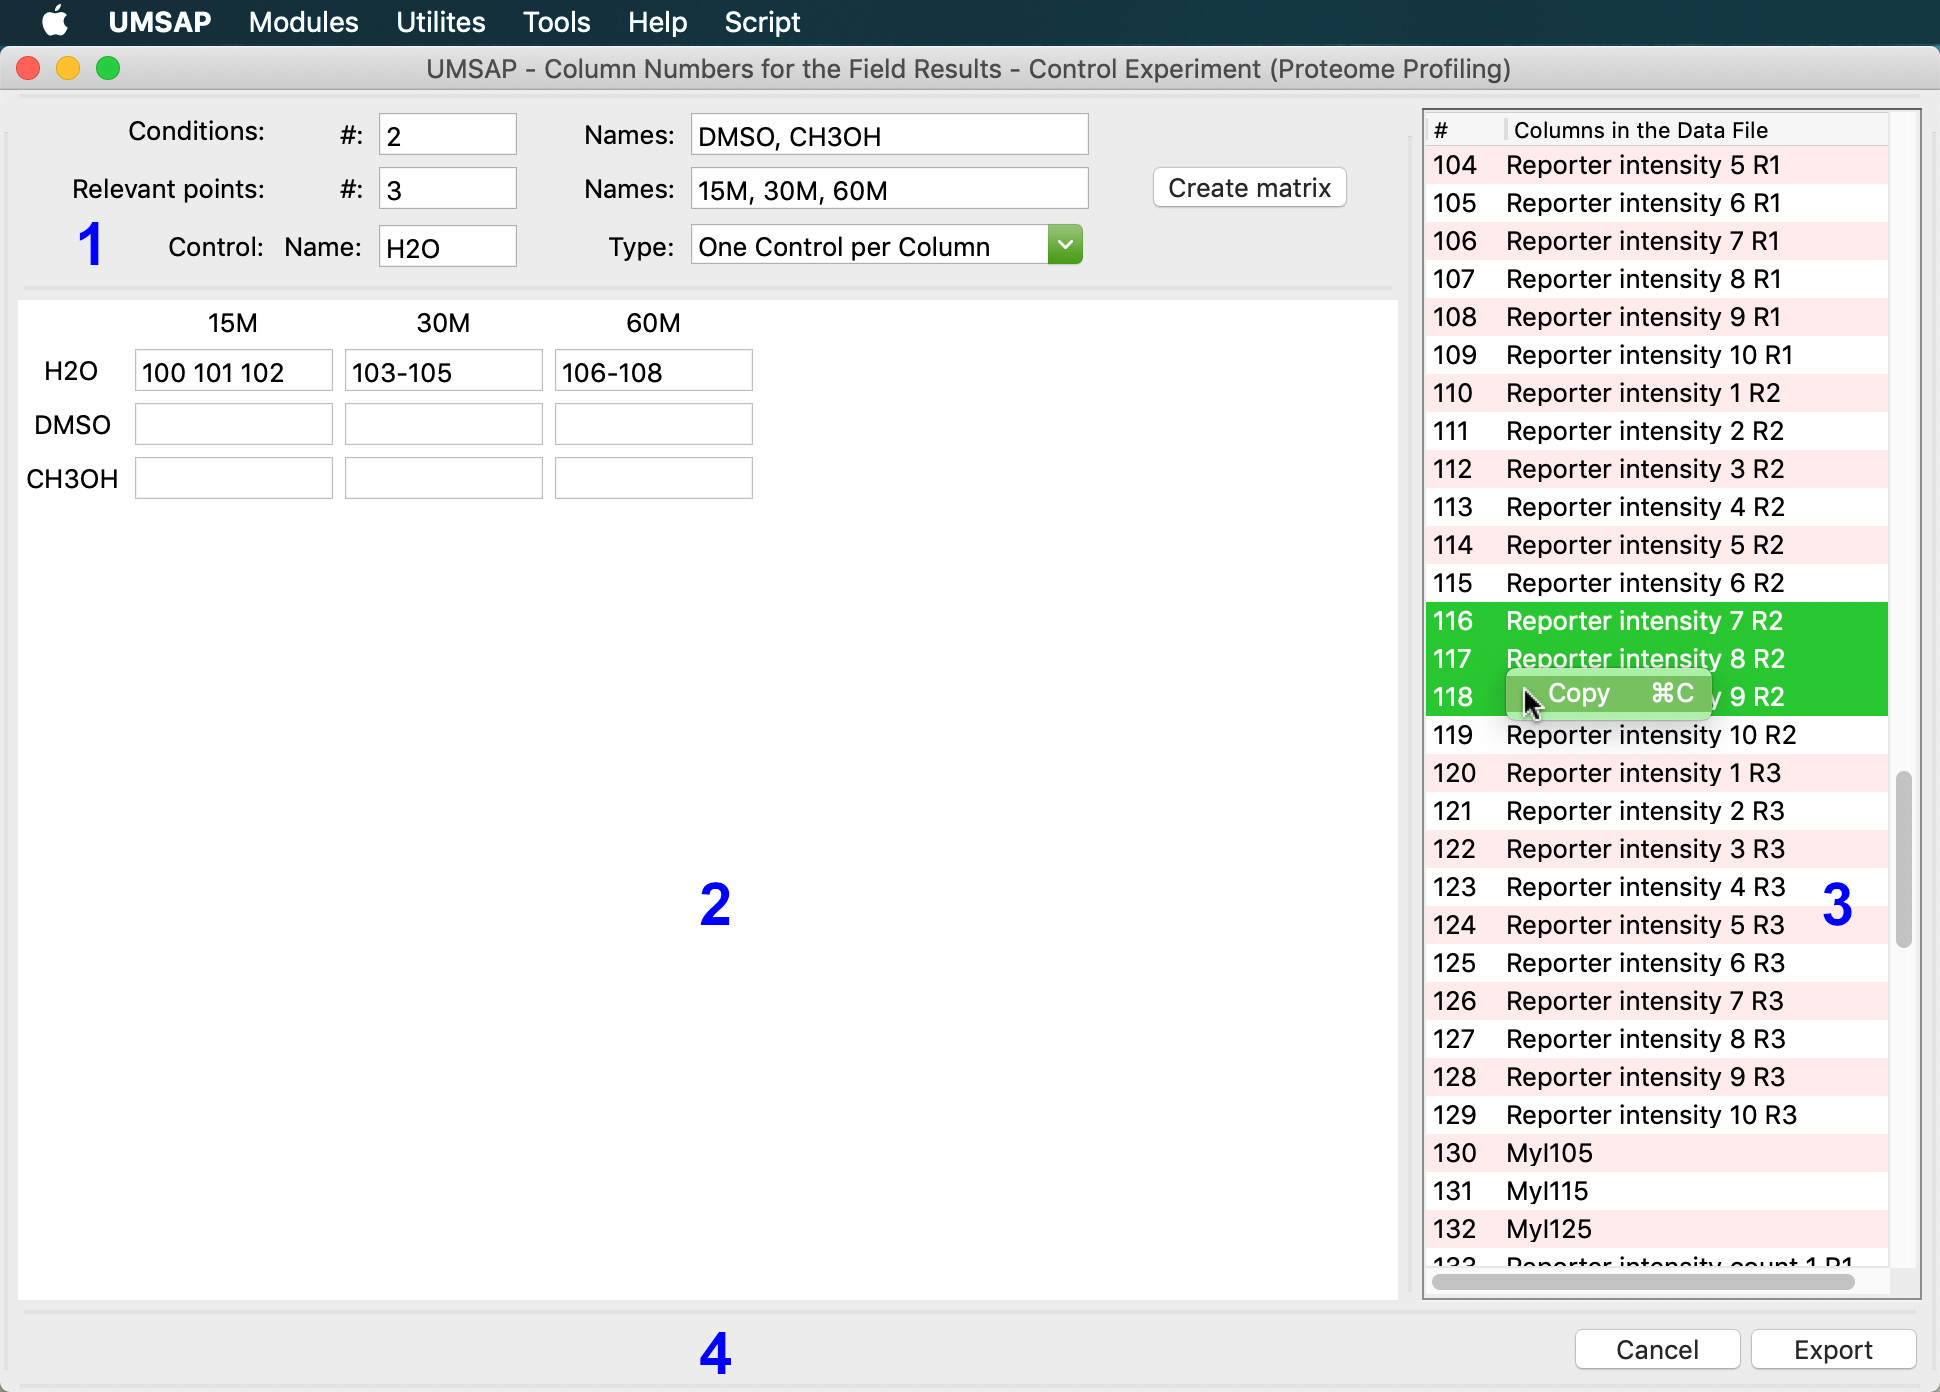
\includegraphics[width=0.7\textwidth]{./IMAGES/MOD-PROTPROF/protprof-rescontrol.jpg}
	\caption[The Result - Control experiments helper window for the Proteome Profiling module]{\textbf{The Result - Control experiments helper window for the Proteome Profiling module.} This window allows users to specify the column numbers in the Data file containing the MS results for the selected conditions, relevant points and control experiments.} 
	\label{fig:protprofResControlWindow}
	\vspace{-5pt} 	
\end{figure}

The column numbers, the labels for conditions, relevant points and control experiments and the information for the controls can also be loaded from a .txt file. The format of the file content is very simple. The first four lines give the values for the labels and control and the rest of the lines specify the column numbers with a comma (,) separating the values for a different condition - relevant point. The following is an example for two conditions, two relevant points and one control for each condition:

Control type : One Control per Row\newline
Control name : MyControl\newline
Condition names: DMSO, H2O\newline
Relevant point names: 30min, 1D\newline
\newline
105 115 125, 106 116 126, 101 111 121  \newline
130 131 132, 108 118 128, 103 113 123\newline

The values for Control type are the same as in the helper window.

Region \num{3} of the Proteome Profiling module main window contains a list box that will display the number and name of the columns found in the Data file. The list box is automatically filled when the Data file is selected. Selected columns in the list box can be directly added to any field in section Column numbers of Region \num{2} of the interface using the right mouse button over the list box or the Tools menu.

Region \num{4} contains two buttons and the progress bar. The Help button leads to an online tutorial while the Start analysis button will trigger the processing of the Data file. The progress bar will give users a rough idea of the remaining processing time after the analysis is started.

\subsection{The Tools menu}

The tools menu in the module window allows to copy the selected columns in the list box in Region \num{3} of the interface to the fields of section Column numbers of Region \num{2} of the interface. The list box in Region \num{3} of the interface can also be cleared. In addition, through this menu users can create a .uscr file with the given options to the module before running the analysis. If something goes wrong during the analysis having the .uscr file means that users do not have to type the values of all the parameters again, see \autoref{subsec:utilUscrFile} for more details.   

\section{The analysis}
\label{sec:protprofTTest}

First, UMSAP will check the validity of the user provided input. In particular, all experiments need to have the same number of replicates as the respective control. Then, the Data file is processed as follow. All proteins found in the Exclude proteins columns are discarded. Proteins that were not identified in all conditions are discarded. Finally, all proteins with a Score value lower than the defined threshold are removed. The intensity values of the remaining proteins are normalized and then a median correction is applied to each experiment if Median correction was selected in section Values. With the resulting intensity values the fold change for each protein and experiment as well as the intensity ratios with respect to the control experiments are calculated and two different analysis are performed.

The fold change is calculated as: 

\begin{equation}
\label{eq:protprofFC}
FC = ave(I_{C, RP}) / ave(I_{Control})
\end{equation}

The first analysis is a t-test to determine if each experiment is significantly different to the corresponding control. The second analysis is a t-test, or ANOVA test if more than two conditions are studied, to determine if the values for the studied conditions are significantly different for each selected relevant point.

Finally, the corrected p values are calculated.

\section{The output files}

The Proteome Profiling module generates up to three files and a folder named Data\_Steps, see \autoref{fig:protprofOutFolder}. The folder Data\_Steps contains a step by step account of all the calculations performed so users can check the accuracy of the calculation or perform further analysis. The files inside Data\_Steps are plain text file with tab separated columns. The first line contains the name of the columns in the file.  

\begin{figure}[h]
	\centering
	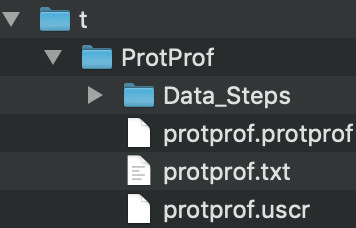
\includegraphics[width=0.35\textwidth]{./IMAGES/MOD-PROTPROF/protprof-files.jpg}	    
	\caption[The structure of the Output folder from the Proteome Profiling module]{\textbf{The structure of the Output folder from the Proteome profiling module.} The file protprof.txt will be created only if requested.} 
	\label{fig:protprofOutFolder}
	\vspace{-5pt} 	
\end{figure}

The three files created have extension .txt, .uscr and .protprof. The file with extension .txt contains all the lines in the Data files but only the columns specified with the parameter Columns to extract in section Column numbers of Region \num{2} of the Proteome Profiling module. This file is generated only if the value of the parameter Columns to extract is not NA. 

The file with extension .uscr contains all the input given by the user so a new analysis may be performed without typing all the option values again, see \autoref{subsec:utilUscrFile}. 

The file with extension .protprof is the main output of the module. This file contains all the results and can be used to generate the graphical representation of the results.    

\section{Visualizing the output files}

After creating the .protprof at the end of the analysis, the Proteome Profiling module will automatically load the file and create a windows to display the results, see \autoref{fig:protprofResultsWindow}. This window is divided in four Regions. 

\begin{figure}[h]
	\centering
	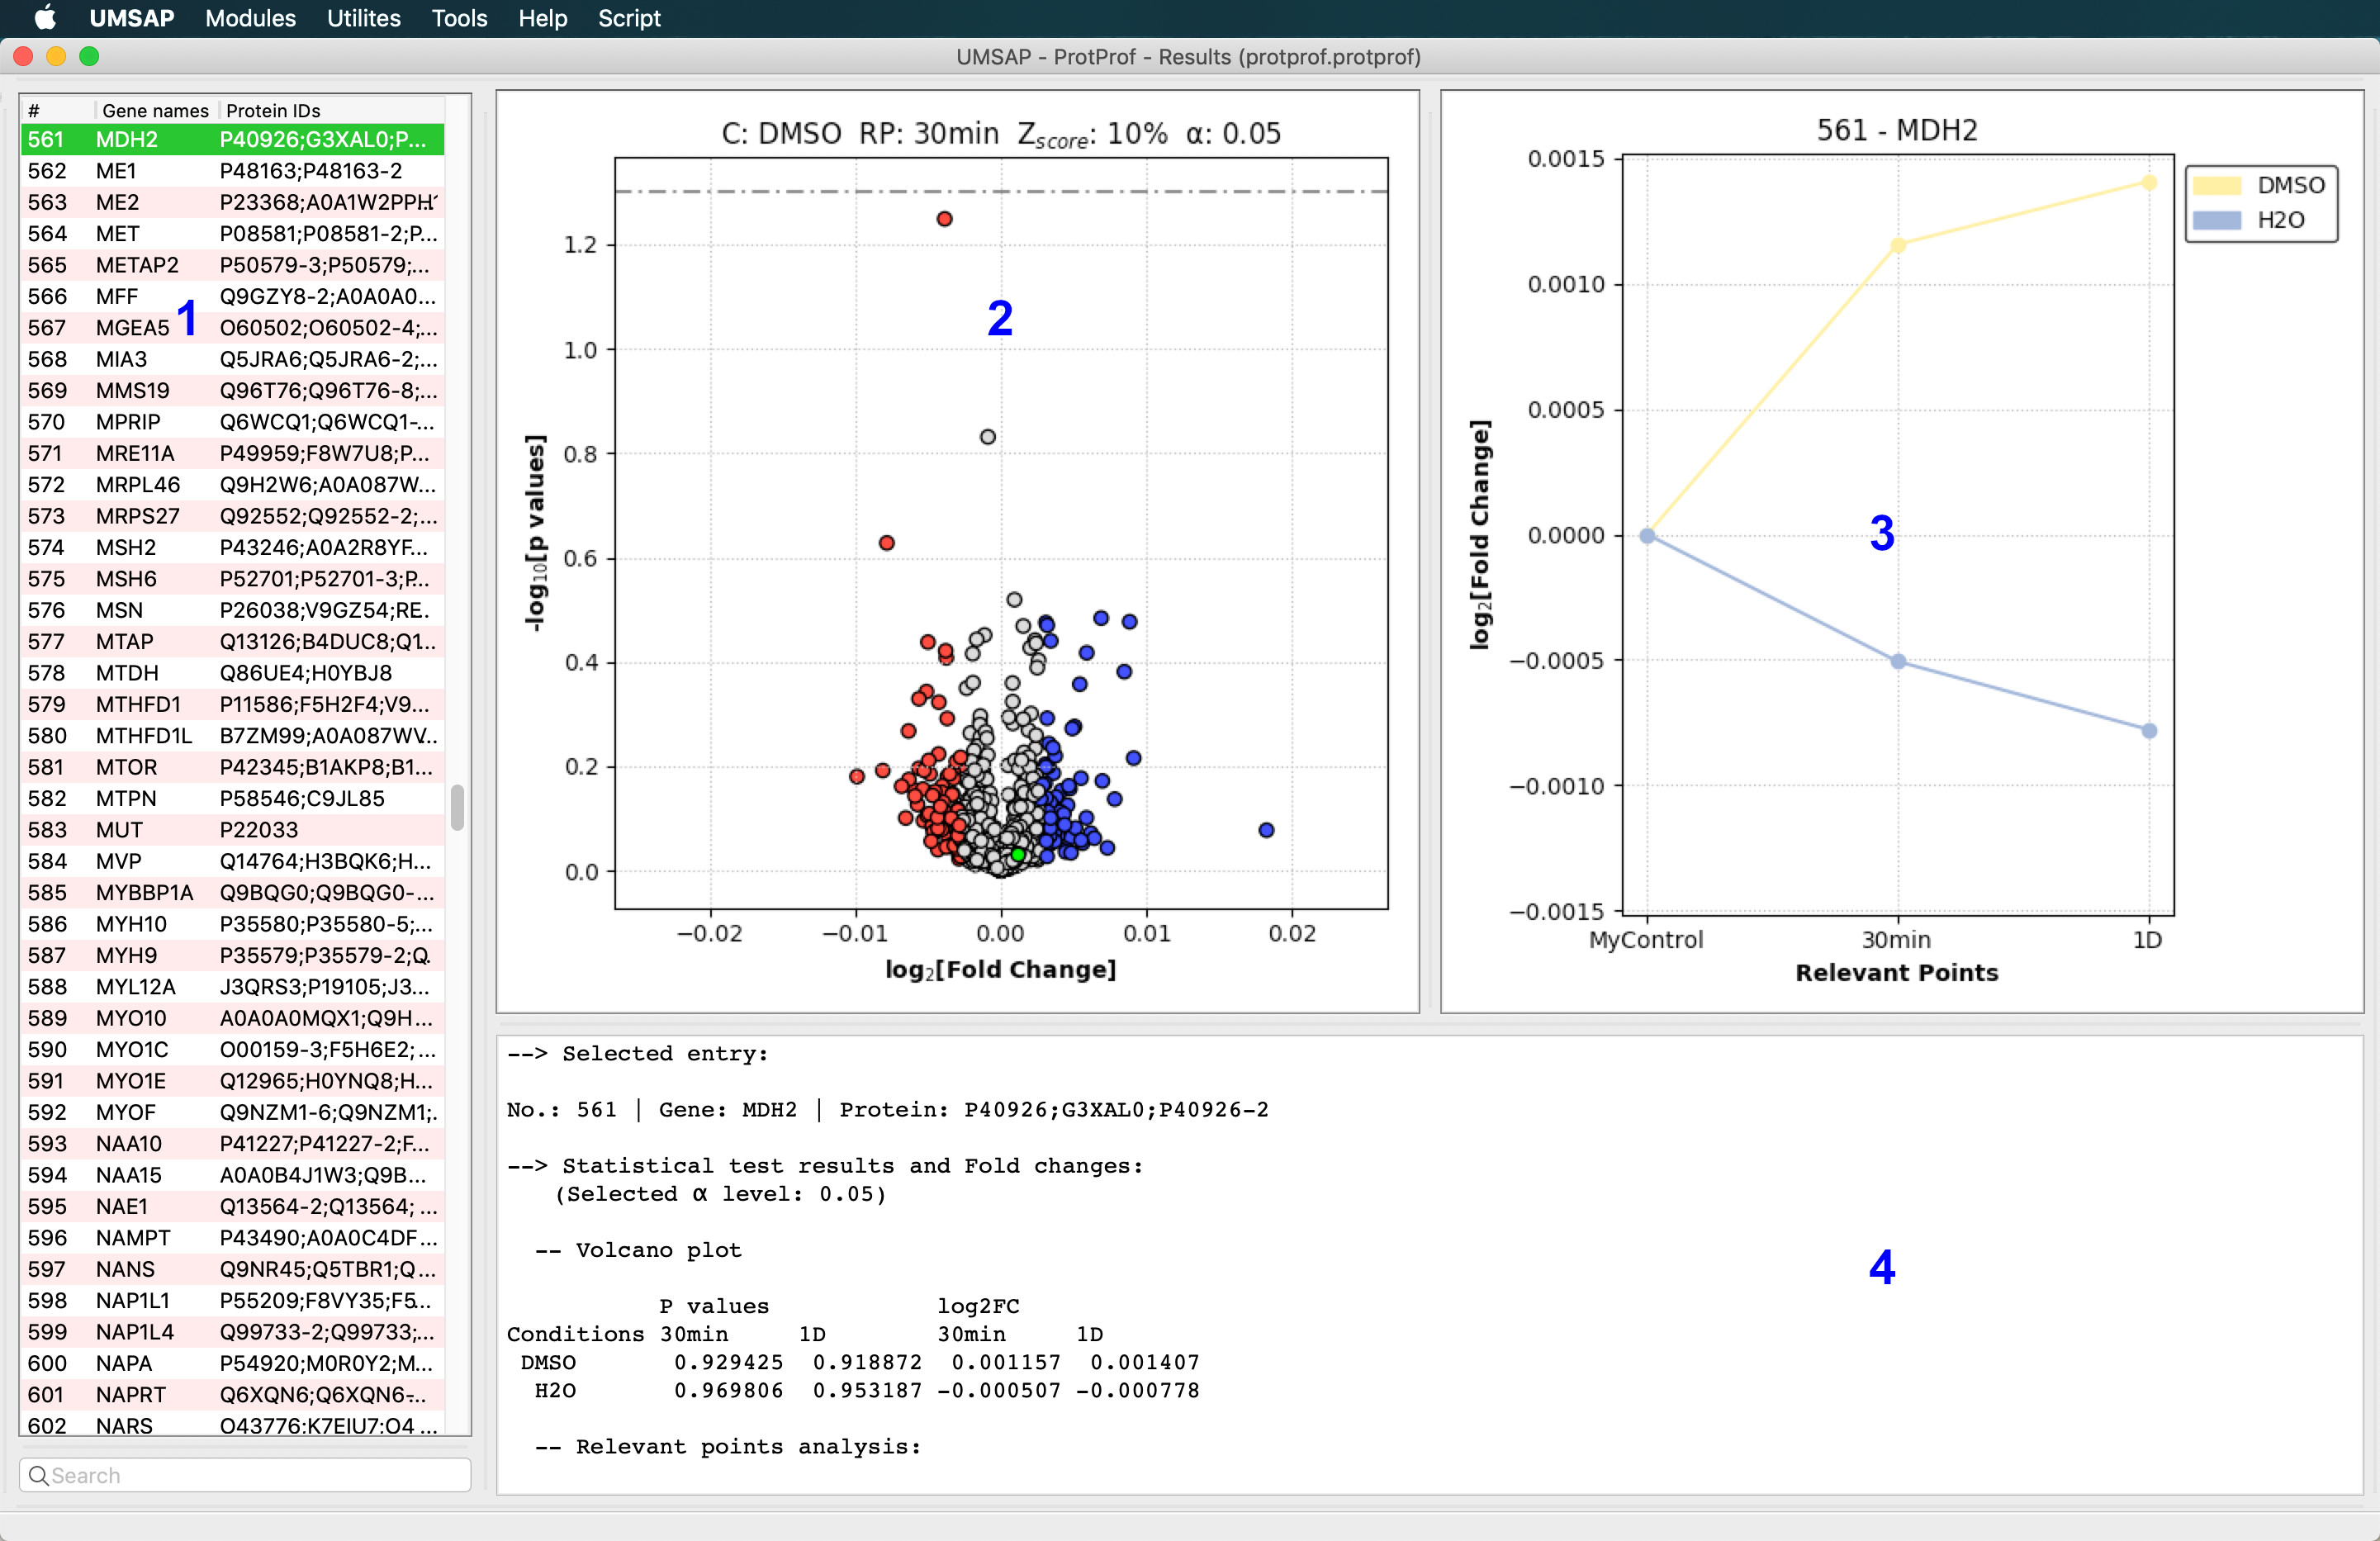
\includegraphics[width=0.8\textwidth]{./IMAGES/MOD-PROTPROF/protprof-frag.jpg}	    
	\caption[The Proteome Profiling analysis window]{\textbf{The Proteome Profiling analysis window.} Users can performed here the analysis of the proteome profiling.} 
	\label{fig:protprofResultsWindow}
	\vspace{-5pt} 	
\end{figure}

Region \num{1} contains a list of all protein IDs and Gene names contained in the .protprof file being shown. The search box at the bottom allows to search for a protein in the list. Selecting a protein in the list will highlight the protein in Region \num{2} and display information about it in Regions \num{3} and \num{4}.

Region \num{2} contains a volcano plot showing the results for the t-test comparing the condition (C), relevant point (RP) to the corresponding control. The volcano plot has a horizontal line indicating the chosen significance level. In addition, the points in the plot can be colored by Z-score allowing to quickly identified the top up (blue) or down (red) regulated proteins. In \autoref{fig:protprofResultsWindow}, the top \SI{10}{\percent} up and down regulated proteins are colored and $\alpha$ is set to 0.05. Selecting a protein in the plot will highlight the selected protein in Region \num{1} and display information about it in Regions \num{3} and \num{4}. See \autoref{sec:protprofTools} for more options.

Region \num{3} contains a plot of $log_2[FC]$ vs Relevant points. The plot allows to see the behavior of the FC along the relevant points for each condition tested in the experiments. See \autoref{sec:protprofTools} for more options.

Region \num{4} shows a summary of the results for a selected proteins. Proteins can be selected in the listbox in Region \num{1} or in the volcano plot of Region \num{2}. The information includes a summary of the selected protein including the number of the protein in the listbox, the gene name and the protein id. Calculated p and $log_2[FC]$ values as well as averages and standard deviations for intensities and ratios.

\subsection{The Tools menu}
\label{sec:protprofTools}

The Tools menu for the results window of the Proteome Profiling module allows to further customize the plots and to apply different filters to the protein list shown in the window.

Under the menu entry Volcano Plot, users can change the condition and relevant point shown in the volcano plot, the Z score value used to color the points in the plot and the $\alpha$ value. An image of the volcano plot can also be created. If the condition or relevant point displayed is changed the Apply Filters menu entry allows to recalculate the filters for the current condition, relevant point displayed.

Under the menu entry Relevant Points, users can show all the proteins at once with different or the same colors and create an image of the Relevant Points graph.

The menu entry Export Data can be used to export the data shown in the window to a plain text file (see \autoref{subsec:utilExpData}) while the Corrected P values entry will display the information in the .protprof file using the corrected p values instead of the regular p values.

\subsubsection{Filters}

The menu entry Filters allows to Add or Remove the filters applied to the protein list. The idea behind Filters is to identify proteins with a desired behavior and discard the rest of the proteins from the listbox in Region \num{1} and the plots in Regions \num{2} and \num{3}. Filters are applied to the current Condition and Relevant point shown in the Volcano plot in Region \num{2}. If the Condition or the Relevant point shown is changed, the new plot will show the proteins obtained after the filter was applied. This allows to follow the behavior of the filtered proteins in all Conditions and Relevant points. The menu entry Applied Filters in the Volcano plot submenu allows to recalculate the filters based on the new Conditions and Relevant point shown. Any number of filters can be applied. The applied filters are shown in the bottom left corner of the results window. 

Filter can be removed in any given order using the menu entry Any in the Remove filter submenu. Additionally, the last applied filter can be removed with the menu entry Last Added or the shortcut Ctrl/Cmd + Z.

Currently, the implemented filters are:

\textbf{\textit{\underline{Z score}}}

This menu entry allows to filter proteins by the Z score value of the Fold change. 

\textbf{\textit{\underline{Log2FC}}}

This menu entry allows to filter proteins by the absolute value of the $log_2[FC]$. 

\textbf{\textit{\underline{P value}}}

This menu entry allows to filter proteins by the p value calculated for the comparison of the currently displayed  Condition and Relevant point to the control experiment. The threshold p value can be given in the 0 to 1 range or as a $-log10$ value. Regular or corrected P values can be used in the filter.

\textbf{\textit{\underline{$\alpha$ value}}}

This menu entry allows to filter proteins by the p values calculated for the comparison of the relevant points. The returned list of proteins consists of proteins for which the calculated p value is less than the selected $\alpha$ value, for at least one relevant point.

\textbf{\textit{\underline{Monotonic}}}

This menu entry allows to filter proteins by the behavior of the $log_2[FC]$ along the Relevant points. The filter searches for proteins that have a monotonically increasing or decreasing (or both) behavior for the condition shown in the Volcano plot. 

\textbf{\textit{\underline{Divergent}}}

This menu entry allows to filter proteins by the behavior of the $log_2[FC]$ along the Relevant points. In this case, the filter searches for proteins that have a monotonically increasing and decreasing behavior in at least two of the conditions tested.




































